\chapter{Thermochronology}

The temperature sensitivity of the K-Ar system (Section
\ref{sec:K-Ar}) is a characteristic feature not only of this method,
but of a separate class of geochronometers known as
`thermochronometers'.  The most important of these methods are the
U-Th-He \ref{sec:U-Th-He} and fission track \ref{sec:fission-tracks}
techniques, which are becoming increasingly popular as a means of
investigating Earth surface processes.

\section{The U-Th-He method}
\label{sec:U-Th-He}

When U and Th decay to various isotopes of Pb (Section
\ref{eq:UThdecay}), they do so by $\alpha$-emission (Section
\ref{sec:radioactivity}). When $\alpha$ particles acquire electrons,
they become helium atoms. Thus, not only Pb content, but also the He
content increases relative to U and Th through time, forming the basis
of the U-Th-He chronometer:
\begin{equation}
\begin{split}
  \left[^4\mbox{He}\right] = &
  \left[8 \frac{137.818}{138.818} (e^{\lambda_{238}t} - 1) +
    7 \frac{1}{138.818} (e^{\lambda_{235}t} - 1) \right] \mbox{[U]} +\\
  ~ & 6 (e^{\lambda_{232}t} - 1) \mbox{[Th]} +
  0.1499 (e^{\lambda_{147}t} - 1) \mbox{[Sm]}
\end{split}
\label{eq:U-Th-He}
\end{equation}

\noindent where [\textsuperscript{4}He], [U], [Th] and [Sm] are
concentrations in atoms or moles per unit mass or volume.  The values
`8', `7' and `6' refer to the number of $\alpha$-particles produced in
the decay chains of $^{238}$U, $^{235}$U and $^{232}$Th, respectively
(Figure \ref{fig:U-Th-series}), 137.818 is the $^{238}$U/$^{235}$U
ratio of naturally occurring uranium in accessory minerals, and the
last term accounts for the (often negligible) accumulation of helium
by Sm-decay (Section \ref{sec:Sm-Nd}). It was Ernest Rutherford who
first proposed that the U-Th-He decay scheme could be used as an
absolute dating technique, making it the oldest radiometric
chronometer. Early experiments on uraninite (UO$_2$) by Robert John
Strutt (4$^{th}$ Baron Rayleigh) at Imperial College London in 1905
yielded ages that were systematically too young. This was correctly
attributed to the volatile nature of the helium atom, which diffuses
out of most minerals at low temperatures and therefore yields only
\emph{minimum ages}. As a result, the method was largely abandoned
until 1987, when American geochronologist Peter Zeitler realised that
this `leaky' behaviour provided a powerful means of reconstructing the
thermal evolution of rocks and minerals. \\

Let C(x,y,z) be the He-concentration as a function of the spatial
coordinates x, y and z.  The evolution of C with time (t) is given by
the diffusion equation (`Fick's law'):
\begin{equation}
\frac{\partial C}{\partial t} = D \left(
\frac{\partial^2C}{\partial x^2} + \frac{\partial^2C}{\partial y^2} +
\frac{\partial^2C}{\partial z^2}\right)
\label{eq:fick}
\end{equation}

Where D is the `diffusion coefficient', which varies exponentially
with temperature (T) according to the `Arrhenius Law':

\begin{equation}
D = D_\circ e^{-\frac{E_a}{RT}}
\label{eq:Arrhenius}
\end{equation}

with D$_\circ$ the `frequency factor', E$_a$ the `activation energy'
and R the ideal gas constant (8.3144621 J/mol.K). By taking the
logarithm of both sides of Equation \ref{eq:Arrhenius}, we obtain
(Figure \ref{fig:Arrhenius}):

\begin{equation}
\ln(D) = \ln(D_\circ) - \frac{E_a}{RT}
\label{eq:logD}
\end{equation}

Both the frequency factor and the activation energy can be determined
from \emph{diffusion experiments}, in which a He-bearing mineral is
subjected to a step-heating experiment similar to the kind we saw in
the $^{40}$Ar/$^{39}$Ar method (Section \ref{sec:Ar-Ar}).\\

Let us now consider the situation of a mineral which (a) accumulates
He through radioactive decay of U and Th, (b) loses He by thermal
diffusion, and (c) undergoes monotonic cooling at a variable rate
dT/dt. At high temperatures, the He will be lost quickly but as time
progresses, the thermal diffusion becomes increasingly sluggish until
the He is eventually `locked' into the crystal lattice and the isotopic
system is effectively \emph{closed}. If the thermal history is so that
1/T increases linearly with time, then it is possible to calculate an
equivalent `closure temperature' T$_c$. This is known as `Dodson's
equation':

\begin{equation}
\frac{E_a}{RT_c} = \ln\left(\frac{ART_c^2D_\circ/r^2}{E_adT/dt}\right)
\label{eq:Tc}
\end{equation}

where r = is the effective grain size (radius) of the mineral and A is
a geometric factor (55 for a sphere, 27 for a cylinder and 8.7 for a
plane sheet). Thus the U-Th-He age calculated at the end of the
aforementioned thermal history equals that which would have been
obtained if He accumulated linearly since the rock passed through
T$_c$.\\

Although the closure temperature concept is an oversimplification of
reality, it has great intuitive appeal. Consider, for example, a
vertical transect in a rapidly exhuming mountain range. The
\emph{apparent} U-Th-He ages along such a transect are approximately
given by the time elapsed since the respective rocks have passed
through T$_c$. For apatite [Ca$_5$(PO$_4$)$_3$(OH,F,Cl)], this is
$\sim 60^{\circ}C$, which corresponds to a depth (assuming a thermal
gradient of 30$^{\circ}$C/km) of 1.5-2km. Thus, the rocks at the high
elevations along the transect will have passed through T$_c$ before
those collected at the bottom of the transect, and the corresponding
U-Th-He ages will therefore increase with elevation. Moreover, the
rate of increase of age increase with elevation can be used to
estimate the \emph{exhumation rate} of the orogen.

\ifpdf
\ifuclnotes
\begin{figure}[!ht]
  \centering
  \def\svgwidth{.9\textwidth}
  \input{Arrhenius.pdf_tex}
  \caption{`Arrhenius' diagram of three step-heating experiments of
    $^4$He in apatite, showing simple diffusion behaviour in agreement
    with Equation \ref{eq:Arrhenius}. Extrapolating the linear trend
    to geological time scales yields a `closure temperature' of
    $\sim$60$^\circ$C (Equation \ref{eq:Tc}). Modified from
    \citet{braun2006}.}
  \label{fig:Arrhenius}
\end{figure}
\else % end of uclnotes
\begin{figure}[!ht]
\noindent\begin{minipage}[t]{.6\textwidth}
\strut\vspace*{-\baselineskip}\newline
\def\svgwidth{\textwidth}
\input{Arrhenius.pdf_tex}
\end{minipage}
\begin{minipage}[t]{.4\textwidth}
  \captionof{figure}{`Arrhenius' diagram of three step-heating
    experiments of $^4$He in apatite, showing simple diffusion
    behaviour in agreement with Equation
    \ref{eq:Arrhenius}. Extrapolating the linear trend to geological
    time scales yields a `closure temperature' of $\sim$60$^\circ$C
    (Equation \ref{eq:Tc}). Modified from \citet{braun2006}.}
  \label{fig:Arrhenius}
\end{minipage}
\end{figure}
\fi % end of pdf
\else
  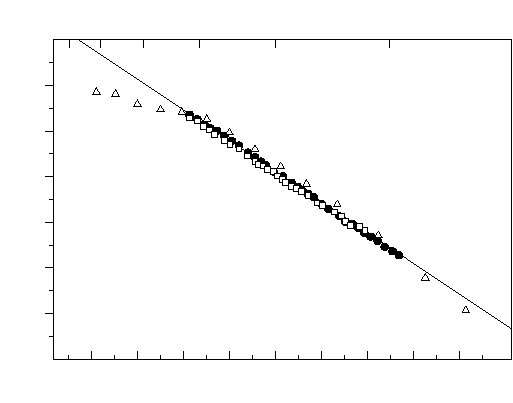
\includegraphics[width=10cm]{../figures/Arrhenius.png}
  \captionof{figure}{`Arrhenius' diagram of three step-heating experiments of
    $^4$He in apatite, showing simple diffusion behaviour in agreement
    with Equation \ref{eq:Arrhenius}. Extrapolating the linear trend
    to geological time scales yields a `closure temperature' of
    $\sim$60$^\circ$C (Equation \ref{eq:Tc}). Modified from
    \citet{braun2006}.}
  \label{fig:Arrhenius}
\fi

\section{Fission tracks}
\label{sec:fission-tracks}

In addition to $\alpha$, $\beta$ and $\gamma$ decay, which form the
basis of the U-Th-Pb (Section \ref{sec:U-Pb}) and U-Th-He (Section
\ref{sec:U-Th-He}) methods, a tiny fraction (1/1,000,000) of the
$^{238}$U atoms decay by \emph{spontaneous fission} (Section
\ref{sec:radioactivity}). In this decay mechanism, the parent nuclide
(i.e., $^{238}$U) decays into two daughter nuclides of roughly equal
mass (e.g., Ba and Kr). These two particles carry a large amount of
energy ($\sim$ 170 MeV) and, having a positive charge, strongly repel
each other. Each of the two fission fragments travels through the
crystal lattice of the host mineral, leaving a trail of damage
behind. Although fission tracks can be directly observed by
transmission electron microscopy (TEM), a more practical approach is
to etch (a polished surface of) the host mineral with acid. This
enlarges the damage zones and makes it possible to count them under an
ordinary petrographic microscope. The volume density $n_s$ (in
cm$^{-3}$) of the fission tracks is given by:
\begin{equation}
n_{s} = \frac{\lambda_f}{\lambda} [^{238}U] \left(e^{\lambda t}-1\right)
\label{eq:Ns}
\end{equation}

where $[^{238}U]$ stands for the volume density the $^{238}$U atoms,
$\lambda_f$ is the fission decay constant
($8.46\times{10}^{-17}$ yr$^{-1}$) and $\lambda$ is the total decay
constant of $^{238}$U ($1.55125\times{10}^{-10}$yr$^{-1}$, see Section
\ref{sec:U-Pb}). The (unobservable) volume density of the tracks is
related to the (observable) surface density $\rho_s$ (in cm$^{-2}$)
by:
\begin{equation}
\rho_s = g_s L n_s
\label{eq:rhos}
\end{equation}

Where g\textsubscript{s} is geometry factor (g\textsubscript{s}=1 if
determined on an internal and g\textsubscript{s}=1/2 on an external
surface) and L is the etchable length of a fission track
($\sim$15$\mu$m). Rearranging Equation \ref{eq:Ns} for time:
\begin{equation}
t = \frac{1}{\lambda}
\ln\left(\frac{\lambda}{\lambda_f}\frac{\rho_s}{[^{238}U] g_s L
}+1\right)
\label{eq:tFT}
\end{equation}

In practice, $[^{238}U]$ is determined by irradiating the (etched)
sample with thermal neutrons in a reactor. This irradiation induces
synthetic fission of $^{235}$U in the mineral (Equation
\ref{eq:235Ufission}). These tracks can be monitored by attaching a
mica detector to the polished mineral surface and etching this monitor
subsequent to irradiation (Figure \ref{fig:EDM}). The surface density
of the induced tracks in the mica detector ($\rho_i$) is a function of
the nuclear cross section of the neutron-induced fission reaction on
$^{235}$U and the neutron fluence in the reactor, both of which are
unknown. A pragmatic solution to this problem is found by irradiating
the sample along with a standard of known age, and lumping all the
unknown parameters together into a calibration factor ($\zeta$), so
that the age of the sample reduces to:
\begin{equation}
t =
\frac{1}{\lambda}\ln\left(1+\frac{g_i}{g_s}\lambda\zeta\rho_d\frac{\rho_s}{\rho_i}\right)
\label{eq:tzeta}
\end{equation}

where $g_s$ = 1, $g_i$ = 1/2 and $\rho_d$ is the surface density of
the induced fission tracks in a dosimeter glass of known (and
constant) U concentration. The latter value is needed to `recycle' the
$\zeta$ value from one irradiation batch to the next, as neutron
fluences might vary through time, or within a sample stack.\\

\ifpdf
\ifuclnotes
\begin{figure}[!ht]
  \centering
  \def\svgwidth{.8\textwidth}
  \input{EDM.pdf_tex}
  \caption{Schematic diagram illustrating the external detector method
    for fission track geochronology \citep[modified
      from][]{galbraith2005}.}
  \label{fig:EDM}
\end{figure}
\else % end of uclnotes
\begin{figure}[!ht]
\noindent\begin{minipage}[t]{.6\textwidth}
\strut\vspace*{-\baselineskip}\newline
\def\svgwidth{\textwidth}
\input{EDM.pdf_tex}
\end{minipage}
\begin{minipage}[t]{.4\textwidth}
  \captionof{figure}{Schematic diagram illustrating the external
    detector method for fission track geochronology \citep[modified
      from][]{galbraith2005}.}
  \label{fig:EDM}
\end{minipage}
\end{figure}
\fi % end of pdf
\else
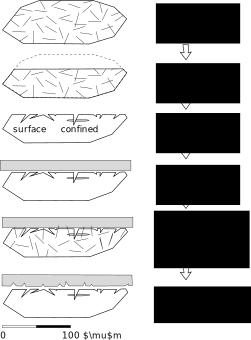
\includegraphics[width=10cm]{../figures/EDM.png}
\caption{Schematic diagram illustrating the external detector method
  for fission track geochronology \citep[modified
    from][]{galbraith2005}.}
  \label{fig:EDM}
\fi

Laboratory experiments have revealed that fission tracks are sensitive
to heat.  For example, it suffices that apatite is heated to
500$^{\circ}$C for 1 hour for all the latent fission tracks to
anneal. Moderate heating shortens the tracks and reduces their surface
density and, hence, the apparent age of the sample. In boreholes, the
apparent fission track age remains constant until a depth is reached
where the ambient temperature is high enough for the tracks to be
reduced in size and number.  This region is called the \emph{Partial
  Annealing Zone} (PAZ). Below the PAZ, no tracks are retained (Figure
\ref{fig:stockli}). The reduction of the surface density of the
spontaneous tracks per unit time can be written as a function of
temperature (T, in Kelvin):

\begin{equation}
\frac{d\rho_s}{dt} = -C \rho_s e^{-E_a/kT}
\label{eq:trackArrhenius}
\end{equation}

where C is a material constant, $E_a$ is the activation energy for
track shortening and k is the Boltzmann constant
(8.616$\times$10$^{-5}$eV/K). Integration of Equation
\ref{eq:trackArrhenius} yields:

\begin{equation}
\ln\left(\frac{\rho_\circ}{\rho}\right) = C~t~e^{-E_a/kT}
\label{eq:lnrho0rho}
\end{equation}

where $\rho_\circ$ is the initial track density prior to
heating. Taking logarithms:

\begin{equation}
\ln(t) = \frac{E_A}{kT} + \ln\left[\ln\left(\frac{\rho_\circ}{\rho}\right)\right] - \ln(C)
\label{eq:lnt}
\end{equation}

For any given \emph{retention coefficient} $\rho_\circ/\rho$, there
exists a linear relationship between ln(t) and 1/T. This is an
\emph{Arrhenius trend} similar to the one described by Equation
\ref{eq:Arrhenius} in the context of U-Th-He thermochronology.  By
extrapolating the Arrhenius diagram to long time scales
($t\sim10^6$yr), it is possible to calculate a `closure temperature'
$T_c$ similar to that which is calculated for the U-Th-He system. For
apatite, T$_c \approx 100^{\circ}C$, whereas for zircon, T$_c \approx
240^{\circ}C$.\\

If a sample has spent some of its time inside the PAZ, then the
subpopulation of its fission tracks formed during that thime will be
shorter than those that subsequently formed above the PAZ. The
probability distribution of the fission track lengths can be
determined by measuring the distance between the two tips of a large
number of (100, say) \emph{horizontally confined} fission tracks under
the optical microscope.  Sophisticated inverse modelling algorithms
have been developed to interpret these length distributions and
extract continuous time-temperature (t-T) paths from them. Such
modelling exercises have become an integral part of modern fission
track studies.

\begin{figure}[!ht]
  \centering
  \ifpdf
  \ifuclnotes
  \def\svgwidth{.9\textwidth}
  \else
  \def\svgwidth{.7\textwidth}
  \fi
  \input{stockli.pdf_tex}
  \else
  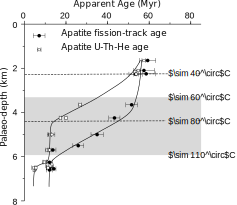
\includegraphics[width=10cm]{../figures/stockli.png}
  \fi
  \caption{Vertical profile of U-Th-He and fission track ages in
    apatite, collected along the footwall of an exhumed normal fault
    block in the White Mountains of eastern California. Samples at the
    highest elevations have resided at shallow depths for up to 55
    Myr. Dashed lines show the extent of the `Partial Retention Zone'
    (PRZ), in which apatite has partially lost its radiogenic
    helium. The grey area indicates the `Partial Annealing Zone',
    where fission tracks have been shortened. At low elevations, young
    ages are observed, indicating rapid exhumation by the normal fault
    at 12 Ma. Additionally, the U-Th-He data show a hint of a second
    exhumation phase at 5 Ma (modified from Stockli, Farley and
    Dumitru, 2000, \textit{Geology} v. 28, no. 11, p. 983-986).}
  \label{fig:stockli}
\end{figure}
